\vspace{-0.5em}
\section{Introduction}
Materialized views (MVs), stored pre-computed results, are a well-studied approach to speed up queries on large datasets \cite{LarsonY85, gupta1995maintenance, chirkova2011materialized}.
During the last 30 years, the research community has thoroughly studied MVs for traditional query processing and recently for more advanced analytics based on linear algebra and machine learning \cite{nikolic2014linview, zhang2014mat}.

However, when the underlying data is changed MVs can become \emph{stale}; the pre-computed results do not reflect the recent changes to the data. 
One solution would be to recompute the MV each time a change occurs; however, in many cases, it is more efficient to incrementally update the MV instead of recomputation.
There has been substantial work in deriving incremental updates (incremental maintenance) for different classes of MVs and optimizing their execution \cite{chirkova2011materialized}.
For frequently changing tables even incremental maintenance can be expensive since every update to the base data requires updating all the dependent views.  
In many important applications, such as summary statistics from user activity logs, new records arrive at a fast rate and data are often distributed across multiple machines making incremental maintenance infeasible. 
As a result, in production environments, it is common to defer view maintenance \cite{chirkova2011materialized, zhou2007lazy, DBLP:conf/sigmod/ColbyGLMT96} so that updates can be batched together to amortize overheads and can be scheduled at times of low system utilization (e.g., nightly).  

While deferring maintenance has benefits, MVs are stale between maintenance periods.
As a result, queries using those MVs can return incorrect answers.
The problem of stale MVs parallels the problem of dirty data studied in data cleaning~\cite{rahm2000data}.
As with dirty data, a stale MV has incorrect, missing, or superfluous rows.
In this work, we explore how answering queries on a stale MV can be formalized as a data cleaning problem. 
%This observation leads us to the main insight behind our work; namely, that a data cleaning approach can be applied to mitigate the negative impacts of deferred MV maintenance.

\begin{figure}[t] \vspace{-2em}
\centering
 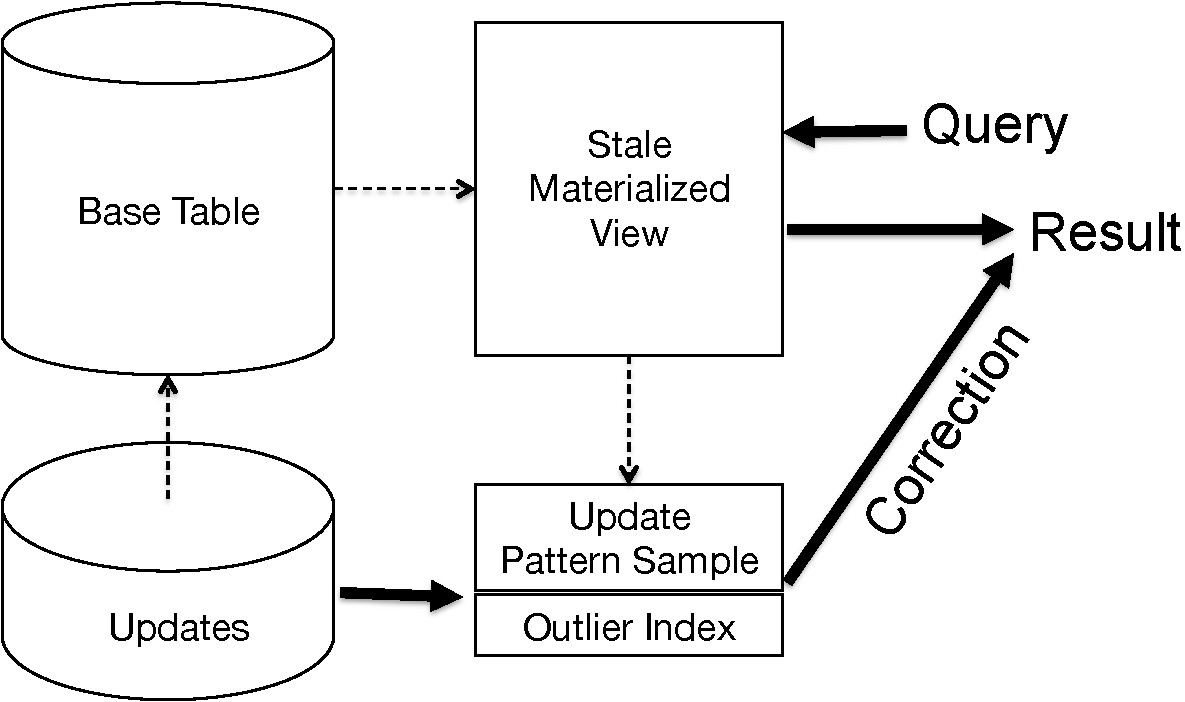
\includegraphics[scale=0.25]{figs/sys-arch.pdf} \vspace{-.25em}
 \caption{Deferred maintenance can lead to stale MVs which have incorrect, missing, and superflous rows. In \svc, we pose this as a data cleaning problem and show that we can use a sample of clean (up-to-date) rows from an MV to correct inaccurate query results on the stale view. We also devise an outlier indexing technique for more accurate corrections in skewed datasets. \label{sys-arch}}\vspace{-1.75em}
\end{figure}

Data cleaning has been studied extensively in the literature (e.g., see Rahm and Do for a survey\cite{rahm2000data}) but increasing data volumes have led to development of new, efficient sampling-based approaches for coping with dirty data.   
In our prior work, we developed the SampleClean framework for scalable aggregate query processing on dirty data \cite{wang1999sample}.
Since data cleaning is often expensive, we proposed cleaning a sample of data using this sample to improve the results of aggregate queries on the full dataset.
Since stale MVs are dirty data, an approach similar to SampleClean raises a new possibility, namely, we can use a sample of ``clean'' rows in the MV to return more accurate query results.

In this paper, we propose \svcfull (\svc), which uses applies data cleaning to stale MVs for fast query processing.
\svc (Figure~\ref{sys-arch}) provides a framework that efficiently cleans a sample of rows from stale MV resulting in a uniform sample of up-to-date rows.
After cleaning, to answer a query, it analyzes how that sample has changed from updates to the base data, and calculates a correction for incorrect query answers on the stale view that compensates for staleness. 
The query results from \svc, while approximate, are up-to-date in the sense that they reflect the most recent data. 
The approximation error due to sampling is more manageable than staleness because: (1) the uniformity of sampling allows us to apply theory from statistics such as the Central Limit Theorem to give tight bounds on approximate results, and (2) the approximate error is parameterized by the sample size which the user can control trading off accuracy for computation.
\svc is complementary to existing deferred maintenance approaches.
When the MVs become stale between maintenance cycles, we apply \svc for query result estimation for a far smaller cost than having to maintain the entire view.

%Both MVs and queries can be complex.

To summarize, our contributions are as follows: (1) we formalize maintenance of a sample MV as a data cleaning operation allowing us to apply SampleClean query processing, (2) we propose efficient techniques to implement the data-cleaning operation, (3) we devise a query processing approach to answer queries accurately using the sample of up-to-date data, (4) we propose an outlier index to increase the accuracy of the approach for power-law, long-tailed, and skewed distributions, and (5) we evaluate our approach on real and synthetic datasets confirming that indeed sampling can reduce view maintenance time while providing accurate query results. 
%\end{itemize}

The paper is organized as follows: 
In Section~\ref{sec-background}, we give the necessary background for our work.
Next, in Section~\ref{sec-arch}, we formalize the problem.
In Sections~\ref{sampling} and~\ref{correction}, we describe the sampling and query processing of our technique.
In Section~\ref{outlier}, we describe the outlier indexing framework.
In Section~\ref{sec:disc}, we discuss limitations and new opportunities of our approach.
Then, in Section~\ref{exp}, we evaluate our approach.
Finally, we discuss Related Work in Section~\ref{related} and present our Conclusions and Future Work in Section~\ref{conclusion}.
We present full versions of our proofs and experimental details in our extended technical report \cite{technicalReport}.
